\documentclass[11pt, oneside]{article}   	% use "amsart" instead of "article" for AMSLaTeX format
\usepackage{geometry}                		% See geometry.pdf to learn the layout options. There are lots.
\geometry{letterpaper}                   		% ... or a4paper or a5paper or ... 
%\geometry{landscape}                		% Activate for for rotated page geometry
%\usepackage[parfill]{parskip}    		% Activate to begin paragraphs with an empty line rather than an indent
\usepackage{graphicx}				% Use pdf, png, jpg, or eps� with pdflatex; use eps in DVI mode
								% TeX will automatically convert eps --> pdf in pdflatex		
\usepackage{amssymb}
\usepackage{amsmath}
\usepackage{color}

\title{Brief Article}
\author{The Author}
%\date{}							% Activate to display a given date or no date

\begin{document}
%\maketitle
\subsection{Vision Based Sensor Overview}
The pinhole camera model, is an approximation of the CMOS machine vision camera that is actually being used. To account for the errors that such an approximation may yield, it is proposed that the \textit{projected} coordinates ($u,v$) be warped with a \textit{radial distortion} as is done in~\cite{dav2002}, in order to obtain a new \textit{distortion} coordinate ($u_d, v_d$) that will better resemble the one which the camera will provide. This radial distortion is mathematically shown as follows%~\cite{distort}:
\begin{equation} \label{eq:raddist}
\begin{split}
u_d - u_0 &= \frac{u-u_0}{(1+k^2_1r^2+k_2r^4)} \\
v_d - v_0 &= \frac{v-v_0}{(1+k^2_1r^2+k_2r^4)}, \\
r &= \sqrt{(u - u_0)^2+(v-v_0)^2}.
\end{split}
\end{equation}
\subsubsection{Camera Calibration}
After using a $9 \times 6$ chessboard pattern for camera calibration in OpenCV \cite{opencv}, the calibration parameters of the camera used in this particular implementation are as follows: $fk_u = fk_v = 520$ pixels, principal point $(u_0,v_0) = (315,239)$ and $K=0.982$ for capture at a resolution of $680\times480$.\\
\subsection{Update Step}
\subsubsection{Measurement Model}
The correction step of the Extended Kalman filter aims to ultimately correct the previously estimated robot pose and landmark position through exterior sensor measurements. With regard to the implementation proposed in this paper, these measurements are obtained through the use of a camera. The measurement process generally involves a measurement estimate that incorporates uncertainty.

\begin{figure}[h] \label{eq:frame}
\begin{center}
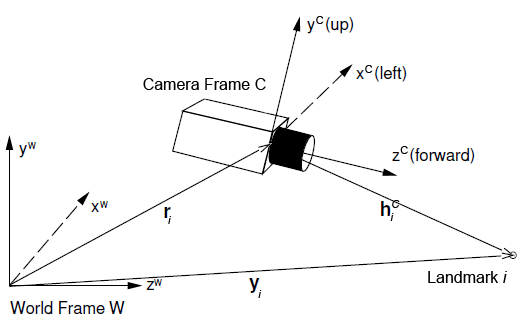
\includegraphics[width=0.8\textwidth, height=0.45\textwidth]{frames_2.png}
\caption{Davison's MonoSLAM representation of the reference frames}
\label{default}
\end{center}
\end{figure}
With reference to figure~\ref{eq:frame}, a feature's cartesian position can be described through a cartesian vector $\textbf{h}^W_i(\boldsymbol{\bar \mu})$, where the feature's cartesian \textbf{point} is shown in relation to the camera's centre: 

\begin{equation}
\textbf{h}^W_{i}(\boldsymbol{\bar \mu}) = \textbf{R}^{CW}\big(\textbf{y}^W_{i}-\textbf{r}^W\big) = 
  \begin{pmatrix}
  \begin{pmatrix}
  x_{i}\\
  y_{i} \\ 
  z_{i} \\
  \end{pmatrix} - \textbf{r}^{W} 
  \end{pmatrix}  
\end{equation}
the subscript $i$ corresponds a directional vector $\textbf{h}^C$ from it's cartesian position $\textbf{r}^W$ to the cartesian position of a given landmark $\textbf{y}^W$.\\\\
A camera however, cannot directly measure a cartesian vector. Instead, a camera measurement (based on the model presented) obtains a vector $\textbf{h}_i$ that is a function of $\textbf{h}^W_{i}$. This vector describes a given feature's horizontal and vertical image positions $(u,v)$. For an undistorted image, the vector $\textbf{h}_i$, more commonly referred to as the measurement function is defined as follows:

 \begin{equation} \label{eq:fmmd}
\textbf{h}_i = 
  \begin{pmatrix}
  u_i \\
  v_i \\ 
  \end{pmatrix} =
    \begin{pmatrix}
  u_0 - fk_u\cfrac{h^R_{i,x}}{h^R_{i,z}}\\
  v_0 - fk_v\cfrac{h^R_{i,y}}{h^R_{i,z}} \\ 
  \end{pmatrix} 
\end{equation}
where $u_0$ and $v_0$ represent the principal point and $fk_u$ and $fk_v$ are the camera calibration parameters described in Appendix~\ref{App:Concepts}.\\
It is evident from the model presented in equation~\ref{eq:fmmd} cannot be directly inverted to obtain a feature's position. The projection of a feature onto the camera's image plane removes any information required to directly obtain the depth of the feature.   
%\subsubsection{}
\subsubsection{Feature Matching}
The following section discusses the measurement of a feature \textit{fully} initialised within the SLAM map. The measurement process seeks to initially estimate the cartesian position of a given feature $\textbf{y}_i$ within the SLAM map. Thereafter, the feature can be compared via a matching sequence. Generally, feature matching is conducted using a normalised cross-correlation search, where a 2D template of the 3D feature is scanned is across the entire image (at each pixel location) until a peak is obtained. MonoSLAM however, seeks to utilise an \textit{active} approach for matching, minimising the the search field and improving efficiency.\\
The EKF inherently contains information that may be utilised in order to prohibit a full cross-correlation search. The measurement function $\textbf{h}({\bar\mu})$ for instance, provides an estimate for a given features location, namely $\textbf{u}_d = ({u}_d,v_d)$. Knowledge of this location therefore allows an active search region to be described within the vicinity of this location. The location estimate of the feature is not the only information regarding the feature that is available as a result of the EKF. Additionally, the uncertainty regarding a given feature's location is stored within the state vector covariance matrix $\textbf{P}_{nN}$. This information can be used to determine the size of the active search region surrounding the location estimate; where the size of the search region is directly proportional to the uncertainty of it's location. If the feature cannot be matched within the aforementioned search region, it cannot contribute to the correction of the robot's pose estimate and is therefore deleted form the SLAM map. The aforementioned process of defining the active search region can be mathematically defined through the \textit{innovation covariance matrix} $\textbf{S}_i$:
\begin{equation}\label{eq:inov}
%\begin{split}
\textbf{S}_i = \frac{\partial\textbf{u}_{d,i}}{\partial\textbf{x}_{v}}P_{xx}\frac{\partial\textbf{u}_{d,i}}{\partial\textbf{x}_{v}}^T + \frac{\partial\textbf{u}_{d,i}}{\partial\textbf{x}_{v}}P_{xy_i}\frac{\partial\textbf{u}_{d,i}}{\partial\textbf{y}_{i}}^T + \frac{\partial\textbf{u}_{d,i}}{\partial\textbf{y}_{i}}P_{y_ix}\frac{\partial\textbf{u}_{d,i}}{\partial\textbf{x}_{v}}^T + \frac{\partial\textbf{u}_{d,i}}{\partial\textbf{y}_{i}}P_{y_iy_i}\frac{\partial\textbf{u}_{d,i}}{\partial\textbf{y}_{i}}^T + \textbf{R}_v
%\end{split}
\end{equation}
The symmetric $2\times2$ matrix $\textbf{S}_i$ represents a 2D Gaussian PDF around the estimated image coordinate. The innovation covariance matrix can then be used to determine an active region the a given feature should lie within. Typically, the active search region is defined to confine within 3 standard deviations (3$\sigma$) of the mean.\\
Furthermore, the innovation matrix provides a measure of the amount of content expected within an eventual actual measurement $\textbf{z}_i$. In the event that many potential measurements are available, features containing a higher $\textbf{S}_i$ present the EKF with more information regarding the camera's position. Candidates for feature estimates are thus chosen according to those that present the most information regarding the position estimate. Feature searches per sampling instance are generally limited (usually about 12 features) due to computational constrains.\\         
Finally, as described in %~\cite{dav2007}
[Davison], an active search will always reduce the area of the template matching search region at the potential \textit{additional} cost of calculating the reduced search region.
\subsubsection{Feature Initialisation}
The inherent disadvantage of a monocular camera, as previously mentioned, is the inability to immediately provide an estimate for the depth of a feature. As a result, a given feature is required to be observed at various viewpoints before its depth can be approximated through a multiple view triangulation. Instead, Davison et al. presents an alternative approach whereby a feature is initialised to lie along an infinite 3D line. This line, originating from the position at which the camera is estimated, extends indefinitely in the direction of the feature. The depth of the feature lies somewhere along the aforementioned line. This depth can be modelled as a uniformly distributed set of discrete depth hypothesis. Briefly, the feature's depth can be interpreted as a 1D probability density, represented only by particle distribution instead. The feature is can then \textit{partially} initialised in the SLAM map as follows:
\begin{equation}
\textbf{y}_{pi} =
\begin{pmatrix}
\textbf{r}_{i}^W \\
 \textbf{\^{h}}_{i}^W \\
\end{pmatrix}
\end{equation}
where $\textbf{r}_{i}^W$ represents the origin of the line and $\textbf{\^{h}}_{i}^W$ is a unit vector representing its direction. The uncertainty describing the aforementioned entities are Gaussian in nature.\\\\
After a feature has been partially initialised, it can be assumed that the feature is re-observed and that each additional observation improves the depth estimate. The particle filter based depth estimation process itself is to a large extent complex, and is explained in more detain in %~\cite{dav0207}
. Intuitively, the depth estimation process can be explained as follows: each particle in the particle set is projected into the image and subsequently matched across each observation. The resulting observations transform the initially uniformly distributed depth probability into one that better resembles a Gaussian density. Once the depth covariance is below a certain threshold, the depth is approximated with a Guassian probability density. Thereafter a feature becomes \textit{fully} initialised, assigned with a standard 3D Gaussian representation.
\subsubsection{Map Management}
Map management forms an integral role in the realisation of the MonoSLAM algorithm. A real-time algorithm, as proposed in this paper, relies on efficient and accurate decisions regarding features within the SLAM map. As a result, a strict protocol is followed in %~\cite{dav0207}
in order to realise a successful real-time algorithm.















     
\end{document}  